\documentclass[12pt]{article}

% This is Rebecca Gill. Welcome to my little template.

% This template is to generate a nice-looking conference paper in
% the style of a mid-2020s political scientist. Once you've 
% written up your paper in the *.Rmd file, you can use this template
% for your conference paper. Then, you can just use a different, 
% journal-specific template to reformat this using a specific 
% journal's submission requirements. Alternatively, using this
% template will give you a *.tex file that you can adjust as needed
% and submit to the journal once they've accepted your manuscript
% for publication. Yay!

% This template is a mashup of the work of many different folks.
% I based most of this on the work of: 
%      Xie et al. and the rest of the rticles package team
%      Steven V. Miller and the templates in his package, stevetemplates
%      Jeffrey Arnold and his psmanuscripts package
% There are other pieces in here from around town, and I cite them in the
% comments wherever I can. My apologies for anyone I've missed here.

% -------------------- Packages -------------------- %

% Font/input basics
\usepackage[T1]{fontenc}
\usepackage[utf8]{inputenc}
\usepackage{lmodern}
%\usepackage{fouriernc}


% Critical math packages
\usepackage{amsmath}
\usepackage{amssymb}
\usepackage{mathtools}

% Tools for theorems, including restatement capability
\usepackage{amsthm}
\usepackage{thmtools}
\usepackage{thm-restate}

% Local table of contents capability
\usepackage{etoc}

% General formatting
\usepackage[margin=1in]{geometry}
\usepackage{float}
\usepackage{setspace}
\usepackage{booktabs}
\setcounter{secnumdepth}{0} % No numbered sections
\usepackage[labelsep=period,font=small,labelfont=bf,margin=5ex]{caption}
%\usepackage{indentfirst} % Indent first paragraph of sections
\usepackage[parfill]{parskip} % Remove all indents

% Bibliography and references
\usepackage{multibib}
\usepackage[sort]{natbib}
\usepackage[bookmarks=false]{hyperref}

% -------------------- Setup -------------------- %

% Don't highlight references/links
\hypersetup{
  colorlinks=true,
  citecolor=black,
  linkcolor=black,
  urlcolor=black
}

% Set up natbib
\bibpunct{(}{)}{;}{a}{}{,}  % citations like (Fearon 1995; Powell 1996, 1999)
\def\citeapos#1{\citeauthor{#1}'s (\citeyear{#1})}  % Sartori's (2002)
\renewcommand{\harvardurl}[1]{\textbf{URL:} \url{#1}}  % less-bad URLs in bibliography
\defcitealias{APSA2018}{APSA 2018}
\newcites{app}{Additional References}

% Theorem environments (add more if needed)
\declaretheorem{lemma}
\declaretheorem{corollary}
\declaretheorem{proposition}

\providecommand{\tightlist}{%
  \setlength{\itemsep}{0pt}\setlength{\parskip}{0pt}}
  
\newcounter{eqset} % Define a separate counter
\renewcommand{\theeqset}{\arabic{eqset}} % Numbering style for the equation set

% Define the command for captioned equation sets
\newcommand{\captionedequationset}[1]{
    \stepcounter{eqset} % Step the equation set counter without affecting references
    \noindent
    \begin{minipage}{\linewidth}
        \centering
        \textbf{Equation Set~\theeqset:} #1
    \end{minipage}
    \vspace{\baselineskip}
    \phantomsection % Create a proper referencing point for hyperref, if used
    \addcontentsline{toc}{equation}{Equation Set~\theeqset: #1} % Add to TOC, if needed
}


% -------------------- Metadata -------------------- %

\title{Debunking the Erroneous Claims of Election Fraud in 2024 Primary Election in Washoe County, Nevada%
  \thanks{The authors write on behalf of themselves. Nothing in this report should be read as speaking for any institution with which Professor Gill or Professor Zorn are associated. This manuscript is currently under development. Please do not cite this working paper without express permission from the authors.}}

% author block code adapted from 
% dtholmes@mail.ubc.ca post on the lab-r-torian

    \usepackage{authblk}
                                        \author[1]{Rebecca Gill, Ph.D.}
                                                            \affil{University of Nevada Las Vegas \thanks{\href{mailto:rebecca.gill@unlv.edu}{\nolinkurl{rebecca.gill@unlv.edu}}}}
                                                                                \author[2]{Christopher Zorn, Ph.D.}
                                                            \affil{Pennsylvania State University \thanks{\href{mailto:zorn@psu.edu}{\nolinkurl{zorn@psu.edu}}}}
                                            
\newlength{\cslhangindent}
\setlength{\cslhangindent}{1.5em}
\newlength{\csllabelwidth}
\setlength{\csllabelwidth}{3em}
\newlength{\cslentryspacingunit} % times entry-spacing
\setlength{\cslentryspacingunit}{\parskip}
\newenvironment{CSLReferences}[2] % #1 hanging-ident, #2 entry spacing
 {% don't indent paragraphs
  \setlength{\parindent}{0pt}
  % turn on hanging indent if param 1 is 1
  \ifodd #1
  \let\oldpar\par
  \def\par{\hangindent=\cslhangindent\oldpar}
  \fi
  % set entry spacing
  \setlength{\parskip}{#2\cslentryspacingunit}
 }%
 {}
\usepackage{calc}
\newcommand{\CSLBlock}[1]{#1\hfill\break}
\newcommand{\CSLLeftMargin}[1]{\parbox[t]{\csllabelwidth}{#1}}
\newcommand{\CSLRightInline}[1]{\parbox[t]{\linewidth - \csllabelwidth}{#1}\break}
\newcommand{\CSLIndent}[1]{\hspace{\cslhangindent}#1}


\begin{document}

% -------------------- Title page -------------------- %

\setcounter{page}{0}
\maketitle
\begin{abstract}
\noindent On July 8, 2024, Robert Beadles posted a message on the website for his Operation Sunlight organization that purports to contain evidence of data manipulation in the 2024 Nevada primary election in Washoe County, NV. In this manuscript, we explain why the claims of fraud are not substantiated by the evidence provided by Mr.~Beadles and his associates.
\end{abstract}
\thispagestyle{empty}

% -------------------- Paper body -------------------- %

\clearpage
\doublespacing

\subsection{Executive Summary}\label{executive-summary}

On July 8, 2024, Robert Beadles posted a message on the website for his Operation Sunlight organization that purports to contain evidence of data manipulation in the 2024 Nevada primary election in Washoe County, NV. The evidence provided made the following claims:

\begin{enumerate}
\def\labelenumi{\arabic{enumi}.}
\tightlist
\item
  \emph{The Vote Share Equations.} There are equations that predict the vote share of a candidate in the non-election day vote election using only (a) that candidate's share of the early vote (b) the other candidate's share of the mail vote, and (c) the total number of votes cast, implying fraud.
\item
  \emph{The Processing Time Graphs.} The fact that the percentage of mail ballots for the Republican Primary as a percentage of the total votes processed at time \emph{t} lagged behind the percentage of mail ballots for the Nonpartisan and Democratic Primary until most ballots were processed implies fraud.
\item
  \emph{The Identical Precincts Analysis.} There are identical total ballot counts across precincts, identical vote proportions for candidates across precincts, identical election day proportions across precincts, and identical mail-in proportions across precincts, all of which suggest fraud.
\end{enumerate}

We have conducted a good faith analysis of all three of these sets of claims. In each case, we have found no evidence of fraud or other malfeasance in the ballot processing in the 2024 Primary Elections. In the report, we attempt to explain the way that the evidence presented on the Operation Sunlight website is undermined by faulty assumptions, misinterpretations of the methodology employed, and AI-generated analysis of simulated (i.e., not real) data. We make the following findings:

\begin{enumerate}
\def\labelenumi{\arabic{enumi}.}
\tightlist
\item
  \emph{As to the Vote Share Equations:} The findings of the linear regression models underpinning these equations show what we would expect them to show, given that the component parts of the vote share are included in the linear predictor. The high significance of the predictors and the high proportion of variance explained by the equations is exactly what we would expect when you try to explain the total vote share (the dependent variable) using its component parts (the independent variables). This does not imply fraud.
\item
  \emph{As to the Processing Time Graphs:} {[}under development{]}
\item
  \emph{As to the Identical Precincts Analysis}: The analysis conducted via ChatGPT and presented in the report is not actually an analysis of the underlying data, but instead is an analysis of data simulated by ChatGPT to produce the very result that the AI's interlocutor demanded that it produce. An analysis of the actual voter files shows no such patterns in the election returns. {[}under development{]}
\end{enumerate}

\subsection{The Vote Share Equations}\label{the-vote-share-equations}

Among the documentation presented in the July 8, 2024, blog post by Beadles is a series of content created by Edward Solomon. The argument regarding the 2024 Washoe County primary election is presented by Solomon is recapped in the ``13.4 Sigma'' report (Solomon 2024). The argument presented here is that, because he was able to predict the total vote share of one candidate by knowing the two proportions of votes by type---and without without knowing the relative percentages of early and mail votes counted in the precinct, this means that the election was rigged. While Solomon claims to be using simple math to prove this claim, this claim relies upon (1) a misunderstanding of the implications of the statistics underlying his calculations, and (2) faulty assumptions about the relative use of mail and early vote methods in Nevada post-2020.

\subsubsection{Solomon's Math}\label{solomons-math}

The argument Solomon makes is explained in a YouTube video called ``Fish Tank Paradox'' (Solomon 2023). In it, he focuses on the various components of the non-election day (NED) vote. His main argument is that, because you can create an equation that can provide a good estimate candidate's total vote share without explicitly specifying the relative proportion of votes between early vote ballots and mail-in ballots, the election must have been subject to intentional tampering. We summarize Solomon's presentation below before explaining why this is not the slam-dunk case he asserts it to be.

Solomon begins by defining several pieces of information about the vote share that would be available to precinct workers in any given election. In the video, he alternates among a bunch of different notation for each of the concepts, but we will stick with his first notation to make it easier to follow. Here, let's assume that he's talking about any particular precinct \(k\). For simplicity purposes, we'll leave the \(k\) subscript off of these equations until it's necessary later on in the process. The first five pieces of information about the vote in a two-candidate race between Donald Trump and Joe Biden are as follows:

\begin{quote}
Let \(T_e\) represent the number of early votes marked for Trump and \(T_m\) represent the number of mail-in ballots marked for Trump. Similarly, let \(B_e\) represent the number of early votes marked for Biden and \(B_m\) represent the number of mail-in ballots marked for Biden. Finally, let \(N\) represent the total number of NED votes cast.
\end{quote}

Once we know all of this, we can write some simple equations that characterize their relationship to one another. Because we have the total NED votes as well as each candidate's total number of votes for each NED ballot type (i.e., early and mail), it's possible to define the relationships among them.

\captionedequationset{Standard Model: Variables} \vspace*{-\baselineskip} \begin{align}
x &= \frac{T_e}{T_e + B_e}
\label{eq:x} \\
y &= \frac{T_m}{T_m + B_m}
\label{eq:y} \\
\alpha &= \frac{T_e + T_m}{N} 
\label{eq:alpha} \\
\Omega &= \frac{T_e + B_e}{N}  \label{eq:omega} \\
1 - \Omega &= \frac{T_m + B_m}{N} \label{eq:omega1} \\
z &= \frac{T_m + B_m}{T_e + B_e}
\label{eq:z}
\end{align}

First, \(x\) from equation \eqref{eq:x} represents Trump's share of the early vote ballots. This is expressed as a number between 0 and 1; when multiplied by 100, it represents the percentage of the total early vote ballots that were marked for Trump. Next, \(y\) from equation \eqref{eq:y} represents Trump's share of the mail ballots. As before, this can be expressed as a number between 0 and 1 or it can be expressed as the percentage of mail ballots marked for Trump if multiplied by 100.

As for \(\alpha\) from equation \eqref{eq:alpha}, this represents Trump's share of all of the NED votes. As before, this is a number between 0 and 1 and can be transformed into the percentage of all NED votes that were marked for Trump. Next, \(\Omega\) in equation \eqref{eq:omega} represents the percentage of all NED votes cast as early votes. Because we have already determined that this is a two-candidate race and are setting aside third-party candidates, write-in candidates, and ``none of these candidates'' selections, we can define \(1-\Omega\) as in equation \eqref{eq:omega1}, which is the percentage of all NED votes cast as mail-in votes.

Finally, we have \(z\), which is defined in equation \eqref{eq:z}. This can be interpreted as the ratio of mail ballots to early votes. So, if there were 200 mail ballots and 100 early votes counted at a particular precinct, the ratio of mail ballots to early votes would be 2:1. It's not clear, however, that he ever uses this one in his calculations.

\captionedequationset{The Standard Model} \vspace*{-\baselineskip} \begin{align}
\alpha &= x \Omega + (1 - \Omega) y \label{eq:alpha1} \\
       &= \frac{T_e}{T_e + B_e} \left( \frac{T_e + B_e}{N} \right) + 
          \frac{T_m}{T_m + B_m} \left( \frac{T_m + B_m}{N} \right) \label{eq:alpha2} 
\end{align}

From here, Solomon presents an equation to calculate \(\alpha\) as a function of \(x\), \(y\), and \(\Omega\); we've included this here as equation \eqref{eq:alpha1}. In \eqref{eq:alpha2}, we've substituted in the values for \(x\) as defined in equation \eqref{eq:x}, for \(y\) as defined in \eqref{eq:y}, and for \(\Omega\) and \(1 - \Omega\) as defined in equations \eqref{eq:omega} and \eqref{eq:omega1}, respectively. In words, this equation says that Trump's share of the NED vote is equal to the sum of (1) his share of the early vote times the proportion of NED votes cast as early votes and (2) his share of the mail-in votes times the proportion of NED votes cast as mail-in votes.

This, of course, is pretty straightforward. Although Solomon's presentation can be confusing on account of his frequent notation changes and his use of oily fish tanks as an analogy, the underlying ideas make a good deal of sense. Indeed, we could also make this idea fit better with the way elections tend to happen in Nevada---namely that there are often more than two candidates and there is a ``none of these candidates'' option in state-wide and presidential elections. But this isn't where Solomon takes things.

His next step is to move around some of the proportions to calculate a some additional values. Although the setup for these calculations is a bit confusing in the video, it essentially boils down to this: In the first set of equations, we tended to lump similar groups of observations together. We either put both types of ballots marked for one of the candidates together or we put both candidates' ballots together by which type of ballots they were. Here, though, Solomon makes an argument that there is something about changing the calculations so that they are unintelligible (e.g., lumping Trump's mail ballots together with Biden's early vote ballots) that makes it easier for government officials to ``cheat'' when they tally votes (or, alternatively he may be suggesting here that it makes it easier for them to \emph{hide} the fact that they are cheating).

In any event, Solomon presents some diagrams to try to show how this works, but they muddy the matter. The gist of the diagrams is that they are fashioned as Cartesian coordinate planes. The first of the two diagrams is in the traditional orientation, which he calls ``standard orientation.'' In the second diagram, the plane appears to be oriented the same way, but nevertheless he calls this the ``bastard orientation,'' perhaps because he goes on to switch the groupings of the ballots into seemingly absurd pairings. Although he uses different notation in this section of the video, we'll continue to use the earlier notation for clarity.

\captionedequationset{Bastard Model: Variables} \vspace*{-\baselineskip} \begin{align}
g &= \frac{T_e}{T_e + B_m} \label{eq:g} \\
h &= \frac{T_m}{T_m + B_e} \label{eq:h} \\
\lambda &= \frac{T_e + B_m}{N} \label{eq:lambda} \\
1 - \lambda &= \frac{T_m + B_e}{N} \label{eq:lambda1}
\end{align}

In the above set of equations, Solomon quantifies four different values. First is \(g\), which is Trump's early vote divided by the sum of Trump's early vote and Biden's mail-in vote. In the video (Solomon 2023), Solomon gives this the term ``westside vote'', referencing the figure he uses to describe how this works. Similarly, \(h\) (or Trump's ``eastside vote'') is defined as Trump's mail vote divided by the sum of Trump's mail vote and Biden's early vote. However, in the main summary document (Solomon 2024), these were named according to which type of ballot was the most dominant for each candidate. This meant that \(g\) was called ``Trump's dominant form.'' We think this is because Trump's share of the early vote was much stronger than Biden's, while Biden's share of the mail vote was much stronger than Trump's. It follows, then, equation \eqref{eq:g} measured his share of these ``dominant votes'' because it took the number of his mail votes and weighted it by his mail votes plus Biden's early votes.

From here, Solomon presents the ``bastard orientation'' versions of equations \eqref{eq:alpha1} and \eqref{eq:alpha2}. To form these equations, he simply substitutes in the new variables \(g\), \(h\), and \(\lambda\):

\captionedequationset{The Bastard Model} \vspace*{-\baselineskip} \begin{align}
\alpha &= g \lambda + (1 - \lambda) h \label{eq:lambda2} \\
       &= \frac{T_e}{T_e + B_m} \left( \frac{T_e + B_m}{N} \right) + \frac{T_m}{T_m + B_e} \left( \frac{T_m + B_e}{N} \right) \label{eq:lambda3}
\end{align}

To demonstrate, let's work through one of the examples Solomon presents in his video. The sample data are summarized in Table \ref{tab:solhypo}.

\begin{table}[ht]
\centering
\caption{Data from Solomon's Hypothetical}
\label{tab:solhypo}
\begin{tabular}{cc}
\hline
Variable & Value \\
\hline
$T_e$ & $500$ \\
$B_e$ & $1500$ \\
$T_m$ & $4500$ \\
$B_m$ & $1500$ \\
$N$ & $8000$ \\
\hline
\end{tabular}
\end{table}

From these data, we can calculate the equations for \(\alpha\) using both of his ``orientations,'' which we show in the Standard Model equation set below. This example demonstrates that the answer is the same regardless which equation we use to calculate it; \(\alpha_{std} = \alpha_{bsd} = 0.625\). Either way, Trump's vote share in this example is 65.5\%. All of this is fine, as far as it goes.

\captionedequationset{Trump v. Biden Example: Standard Model} \vspace*{-\baselineskip} \begin{align}
  \alpha_{std} &= x \Omega + (1-\Omega) y \\
         &= \frac{500}{500 + 1500} \times \frac{500 + 1500}{8000} + \frac{4500 + 1500}{8000} \times \frac{4500}{4500 + 1500} \label{eq:hypo1} \\
         &= 0.625
\end{align}

\captionedequationset{Trump v. Biden Example: Bastard Model} \vspace*{-\baselineskip} \begin{align}
  \alpha_{bst} &= g \lambda + (1-\lambda) h \\
        &= \frac{500}{500+1500} \times \frac{500+1500}{8000} + \frac{4500+1500}{8000} \times \frac{4500}{4500+1500} \label{eq: hypo2} \\
        &= 0.625
\end{align}

\subsubsection{Solomon's Models}\label{solomons-models}

Solomon's math checks out here, despite the fact that he probably makes it a lot harder to follow than it needs to be. It's not clear whether or not this is by design as an attempt to muddy the waters, or if the write-up was just hurried. Either way, it's true that the equations he presents are both valid ways to calculate total NED vote share in a simplified two-person race given the component parts: vote totals by candidate and ballot type.

The next section of the video (beginning around the 50 minute mark) is where the error occurs. Here, Solomon shows what happens when you plug real precinct-level election data into this equation using what is essentially ordinary least squares regression (OLS). OLS is a simple but elegant way to find patterns in a dependent variable (here that is \(\alpha\)) using a series of independent variables (here those are the remaining terms in the equation). Doing this yields parameter estimates that characterize the straight lines that one can place in the hyperplane created by treating the parameters defining the patterns as partial slope coefficients in a multivariate OLS model.

Solomon demonstrates this idea without using any OLS models (which I think he refers to as ``woke concepts'' in the video). He generates a three-dimensional plot where each dot represents a single precinct's values for \(x\) (or \(g\)), \(y\) (or \(h\)), and \(\Omega\) (or \(\lambda\)). Then, he demonstrates that the resulting plot has variability on the x-axis and the y-axis, but has very little variability on the z-axis, which is the one that represents early votes as a proportion of all votes at the precinct (or dominant votes as a proportion of all votes at the precinct). It is this lack of a pattern on the z-axis that Solomon points to as evidence that elections have been ``rigged.''

Let's run through the example he uses in the video. He downloads data for the presidential race in the 2020 General Election in Clark County, Nevada. we've used this exact same data to generate the building blocks of the analysis, \(T_e\), \(T_m\), \(B_e\), and \(B_m\). The source code for this document shows that the data are imported directly from the Secretary of State website. The data has vote totals covering a total of 1150 precincts. However, 85 of these precincts reported incomplete vote breakdowns to protect individual voters against the possibility of being identified; this happens because of how few registered voters reside in those precincts. Removing the precincts with incomplete data, we get a total of 1065 precincts.

\begin{table}[!htbp] \centering \renewcommand*{\arraystretch}{1.1}\caption{Summary Statistics}\resizebox{\textwidth}{!}{
\begin{tabular}{lrrrrrrr}
\hline
\hline
Variable & N & Mean & Std. Dev. & Min & Pctl. 25 & Pctl. 75 & Max \\ 
\hline
t\_e & 1065 & 220 & 159 & 0 & 102 & 314 & 1127 \\ 
t\_m & 1065 & 128 & 97 & 0 & 66 & 173 & 844 \\ 
b\_e & 1065 & 161 & 107 & 0 & 93 & 223 & 666 \\ 
b\_m & 1065 & 285 & 175 & 0 & 179 & 386 & 1069\\ 
\hline
\hline
\end{tabular}
}
\end{table}

The NED vote totals for these precincts are summarized in Table 2. From here, we can calculate the values we need to put into Solomon's equations. We've summarized the resulting components in Table 3. At this point, we are ready to estimate some OLS models. Remember that this is where Solomon purports to find his evidence of vote-rigging. He doesn't show the model estimates in his video; he just shows what the parameter estimates are (\(\lambda \approx 0.635\) and \(1-\lambda \approx 0.365\)) and uses those to make some graphs of his model predicting \(\alpha_{bst}\). But we'll go ahead and replicate that part of the analysis here. We'll create two different models: one to identify the parameter estimates for \(\Omega\) and \(1-\Omega\) and the other to estimate \(\lambda\) and \(1-\lambda\). The model equations for the Standard Orientation model and the Bastard Orientation model are presented in equations \eqref{eq:stdols} and \eqref{eq:bstols}.

\begin{table}[!htbp] \centering \renewcommand*{\arraystretch}{1.1}\caption{Summary Statistics}\resizebox{\textwidth}{!}{
\begin{tabular}{lrrrrrrr}
\hline
\hline
Variable & N & Mean & Std. Dev. & Min & Pctl. 25 & Pctl. 75 & Max \\ 
\hline
x & 985 & 0.56 & 0.15 & 0.047 & 0.48 & 0.66 & 1 \\ 
y & 985 & 0.31 & 0.11 & 0.034 & 0.24 & 0.37 & 0.93 \\ 
g & 985 & 0.43 & 0.14 & 0.027 & 0.34 & 0.51 & 0.95 \\ 
h & 985 & 0.45 & 0.15 & 0.043 & 0.35 & 0.52 & 1 \\ 
n & 1065 & 795 & 485 & 0 & 501 & 1069 & 3369 \\ 
omega & 985 & 0.48 & 0.072 & 0.21 & 0.44 & 0.52 & 0.73 \\ 
lambda & 985 & 0.64 & 0.039 & 0.41 & 0.61 & 0.66 & 0.82 \\ 
alpha & 985 & 0.43 & 0.13 & 0.052 & 0.35 & 0.51 & 0.96\\ 
\hline
\hline
\end{tabular}
}
\end{table}

Recall that Solomon's complaint is that he was able to create models where the estimates of these parameters did \emph{not} vary much between precincts. This is why he says that you can predict \(\alpha\) so well without knowing the relative distribution of vote types; just the relative share of each vote type for each candidate. If it is true that \(\Omega\) and \(\lambda\) are very similar across precincts, we should be able to match the parameter estimates from each of these models to the mean of the parameters as they appear in Table 2.

Because we already know their means in the data, we know that we should expect to see something close to \(\Omega \approx\) 0.48 and something like \(\lambda \approx\) 0.64 in these models. If we are in fact able to estimate a value for each of these parameters that is largely constant among precincts, these estimates should be statistically significant (i.e., they should have very small p-values as denoted by a lot of stars next to the estimate) and the model should explain a very high percentage of the variance in the dependent variable (i.e., in Trump's share of the NED votes). We would know the latter is the case if we observe \(R^2\) values that are very close to 1. Because of the way our data are organized, we should also expect that the intercept of the model should be approximately zero.

\captionedequationset{Standard and Bastard as OLS Models} \vspace*{-\baselineskip} \begin{align}
\textrm{Standard Orientation: } \alpha_k &= \Omega x + (1-\Omega) y + \varepsilon \label{eq:stdols} \\
\textrm{Bastard Orientation: } \alpha_k &= \lambda g + (1- \lambda) h + \varepsilon \label{eq:bstols}
\end{align}

\begin{table}
\caption{Statistical models}
\begin{center}
\begin{tabular}{l c c}
\hline
 & Standard & Bastard \\
\hline
(Intercept) & $-0.02^{***}$ & $-0.00^{**}$ \\
            & $(0.00)$      & $(0.00)$     \\
y           & $0.49^{***}$  &              \\
            & $(0.01)$      &              \\
x           & $0.53^{***}$  &              \\
            & $(0.01)$      &              \\
g           &               & $0.64^{***}$ \\
            &               & $(0.00)$     \\
h           &               & $0.37^{***}$ \\
            &               & $(0.00)$     \\
\hline
R$^2$       & $0.98$        & $1.00$       \\
Adj. R$^2$  & $0.98$        & $1.00$       \\
Num. obs.   & $985$         & $985$        \\
\hline
\multicolumn{3}{l}{\scriptsize{$^{***}p<0.001$; $^{**}p<0.01$; $^{*}p<0.05$}}
\end{tabular}
\label{table:coefficients}
\end{center}
\end{table}

Table 4 demonstrates that we \emph{are} able to derive estimates for the parameters \(\Omega\) and \(\lambda\) (and, by definition, \(1-\Omega\) and \(1-\lambda\)). Notice that the intercept term in both equations is approximately zero. The estimate for \(\Omega_{std}=\) 0.49, which is very close to the mean from Table 3. This is exactly what we'd expect. But it's the high \(R^2\), which almost 1, that tells us that this model does a near-perfect job of estimating Trump's NED vote share without us inputting the value of \(\Omega\) into the model.

The story is similar for our estimate of \(\lambda\). In the right-hand column of Table 4, we see that \(\lambda_{bst}=\) 0.64, which is also very close to the mean calculated in Table 3. Although Solomon did not provide us with his OLS-derived estimate of \(\alpha\), he did tell us that his estimate for \(\lambda\) was 0.635, which is very similar to our \(\hat{\lambda}_{bst}\). Again, this parameter estimate is statistically significant and the model explains nearly all of the variance in the estimate of Trump's NED vote share (since \(R^2=1.00\)).

\begin{figure}
\centering
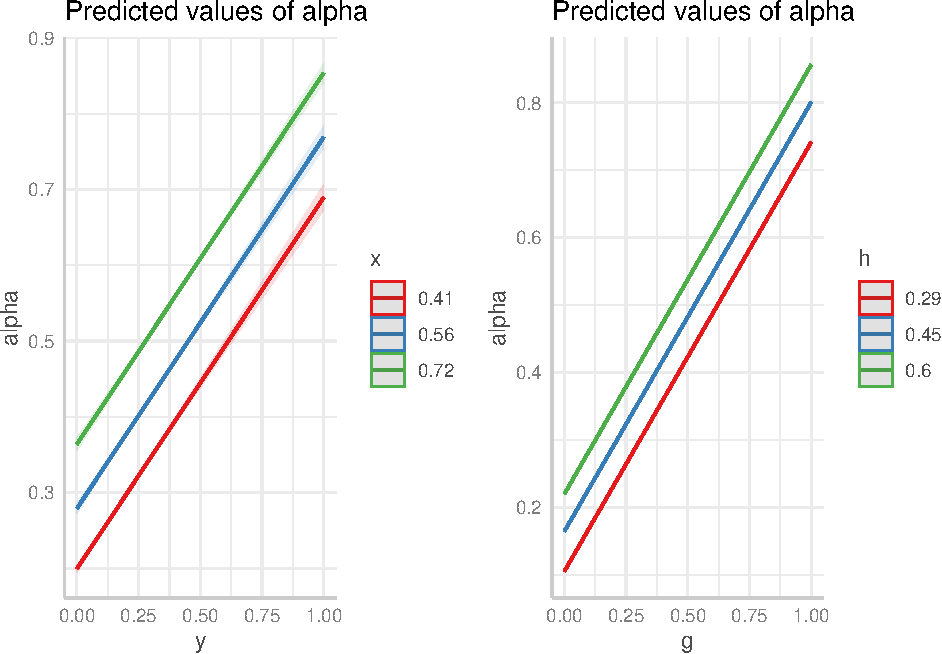
\includegraphics{Report_files/figure-latex/figz2-1.pdf}
\caption{\label{fig:figz2}Predicted Values of Trump Vote Share}
\end{figure}

We can see how this works by looking at plots of the predicted \(\alpha\) values for both of these models. These are presented in Figure 2. In the first plot, we have values of \(x\) at the second quartile, the median, and the fourth quartile in red, blue, and green, respectively. If Trump's share of the early vote (\(x\)) is at its median (the blue line) and his share of the mail votes is about 50\%, his total vote share is expected to be a touch over 50\%. The shaded area around each of the lines represents the confidence interval around these predictions. Given the results from Table 4, the fact that these bands are extremely narrow isn't surprising. This just means that we can be very confident in the estimates of \(\alpha_{std}\) generated by this equation.

The story is very similar in the second plot. Even though the pieces of information we're using to derive the estimate of \(\lambda\) are somewhat nonsensical, we are still able to use that estimated \(\lambda_{bst}\) to predict Trump's share of the NED votes with great precision. This plot shows that, if Trump's share of the subdominant vote \(h\) is about 60\% and his share of the dominant vote \(g\) is about 60\%, we can expect his total NED vote share to be about 65\%.

Taken together, this shows that Solomon \emph{is} correct that the relative percentage of early votes and mail votes is very consistent across Clark County precincts in the 2020 presidential election, as are the relative percentage of dominant votes and subdominant votes in the Bastard Orientation. This isn't anything to be surprised by, as we will explain shortly. First, though, let's apply this same strategy to the Washoe County Primary in 2024.

\subsubsection{Applying Solomon's Math to Washoe County Primary 2024}\label{applying-solomons-math-to-washoe-county-primary-2024}

In the report alleging fraud in the Washoe County 2024 Primary Election (Solomon 2024) (the Report), we see Solomon's math applied to the Reno City Council Ward 5 race and two nonpartisan school trustee primaries (Districts A and D). We'll replicate the analysis of the City Council race here. This race was between four candidates: Browning-Peuchaud (SBP) votes, Cassidy (BMC), Reese (DTR), and Webster (TCW). According to the Washoe County Election Summary Report (\emph{Election Summary Report: Closed Primary, Washoe County} 2024), the vote shares were as follows: TCW with 17.31\%, SBP with 18.10\%, BMC with 27.45\%, and DTR winning with 37.14\%. However, because DTR won with less than 50\% of the vote, the top two vote getters (BMC and DTR) will appear on the general election ballot in November 2024.

The setup for this application of Solomon's math is a bit different from the example in the video. Let's establish some notation to get us started. I'll use candidate initials with the following subscripts: \(m\) for mail vote counts, \(e\) for early vote counts, and \(d\) for election day vote counts. And, although it is certainly possible to reorganize the equations to accommodate this, Solomon reports that ChatGPT recommended to him that he arrange the inputs as in Table \ref{tab:renodata}.

\begin{table}[ht]
\centering
\caption{Terms for RCC Ward 5 Model}
\label{tab:renodata}
\begin{tabular}{cc}
\hline
Term & Content \\
\hline
$A$ & $BMC_e + BMC_d +SBP_d$ \\
$B$ & $DTR_e + DTR_d + BMC_m$ \\
$C$ & $TCW_m$ \\
$D$ & $DTR_m + SBP_m$ \\
$N$ & $A+B+C+D$ \\
\hline
\end{tabular}
\end{table}

Unlike the terms used in the Trump-Biden 2020 example, these combinations of values do not make obvious sense. Solomon does note, rightly, that looking at a sub-county race means that there are very few precincts that can be incorporated into the analysis. This is what is referred to as a ``small-\(n\)'' problem. Having a the same number of variables or more relative to the number of observations (here, precincts) in the data means that the model cannot be estimated. Since we have \(n=17\) districts with all of the relevant information for the analysis, we fall well short of that. However, Solomon also notes that ``the Defense could quickly argue that the model is overfitted'' (Solomon 2024, 4). It is true that complex models on small datasets lack power. It is also true that overfitting can be a real problem, leading to misleading inferences if we're using the model for prediction or hypothesis testing. It is probably wise, then, to try to simplify the model to include only the necessary variables that measure the underlying concepts that we think will help us predict our outcome (here, that's \(\alpha\)). These variables should be sensible, though, and it's not immediately clear from the Report whether this specification makes sense for what Solomon is trying to do.

The next step is to take the voter file from Washoe County and reorganize it to come up with the component parts of these terms. Solomon only uses 16 of the 19 precincts in Ward 5. He doesn't explain why he drops three observations in this race, but his discussion of his School Board Trustee District D race gives us some hints:

\begin{quote}
Primaries are characterized by low voter turnout. In General Elections, precincts with fewer than 200 votes are excluded from analysis to maintain statistical reliability---ensuring errors are minimal, typically within half a percent. Even a precinct with just 50 votes could see a 2\% error if the predictive equation misses just one vote. Therefore, for General Elections, a higher threshold ensures robust analysis. However, applying the same criteria to Primary Elections would leave us with too few precincts to analyze, given their inherently lower turnout. Hence, for primaries, we set a cull threshold at 100 votes, which slightly reduces the \(R^2\) of the \(g\), \(h\), \(\alpha\) equations from 0.99 to around 0.98. \ldots{} Now, will the defense\footnote{This footnote is not included in the original text, but this language deserves a bit of explanation. As far as we can tell, the Report (Solomon 2024) is written in the context of lawsuits alleging election irregularities in court. If this is intended to be evidence of such irregularities, the ``defense'' would probably be the lawyers arguing for the government that the materials presented in the Report do not constitute evidence of cheating, tampering, maladministration of elections, etc.} attempt to argue that I ``cherry-picked'' \ldots{} precincts? Of course they will. (Solomon 2024, 3)
\end{quote}

\begin{table}[!htbp] \centering \renewcommand*{\arraystretch}{1.1}\caption{Summary Statistics}\resizebox{\textwidth}{!}{
\begin{tabular}{lrrrrrrr}
\hline
\hline
Variable & N & Mean & Std. Dev. & Min & Pctl. 25 & Pctl. 75 & Max \\ 
\hline
SBP Early Vote & 16 & 9.9 & 6.8 & 0 & 5 & 15 & 21 \\ 
SBP Election Day & 16 & 12 & 6.9 & 1 & 8.5 & 15 & 24 \\ 
SBP Mail & 16 & 79 & 68 & 1 & 42 & 92 & 267 \\ 
BMC Early Vote & 16 & 22 & 15 & 1 & 11 & 35 & 44 \\ 
BMC Election Day & 16 & 31 & 20 & 0 & 21 & 41 & 79 \\ 
BMC Mail & 16 & 99 & 102 & 1 & 43 & 107 & 390 \\ 
DTR Early Vote & 16 & 24 & 17 & 0 & 12 & 36 & 54 \\ 
DTR Election Day & 16 & 26 & 16 & 1 & 16 & 38 & 48 \\ 
DTR Mail & 16 & 156 & 106 & 1 & 86 & 208 & 402 \\ 
TCW Early Vote & 16 & 8.9 & 7 & 0 & 2.5 & 14 & 21 \\ 
TCW Election Day & 16 & 13 & 9 & 0 & 7 & 19 & 30 \\ 
TCW Mail & 16 & 74 & 48 & 0 & 38 & 108 & 149\\ 
\hline
\hline
\end{tabular}
}
\end{table}

Some descriptive statistics using the remaining 16 precincts can be found in the Table 6. From here, we can calculate the values we need to put into Solomon's model. He has defined the variables for the model this way:

\captionedequationset{Variables for Reno Ward 5 Example} \vspace*{-\baselineskip} \begin{align}
g &= \frac{A}{A+D} \label{eq:greno} \\
h &= \frac{C}{C+B} \label{eq:hreno} \\
\lambda &= \frac{A+D}{N} \label{eq:lreno} \\
1 - \lambda &= \frac{A+C}{N} \label{eq:lreno1}
\end{align}

\begin{table}[!htbp] \centering \renewcommand*{\arraystretch}{1.1}\caption{Summary Statistics}\resizebox{\textwidth}{!}{
\begin{tabular}{lrrrrrrr}
\hline
\hline
Variable & N & Mean & Std. Dev. & Min & Pctl. 25 & Pctl. 75 & Max \\ 
\hline
A & 16 & 65 & 39 & 2 & 42 & 88 & 141 \\ 
B & 16 & 149 & 119 & 5 & 83 & 190 & 451 \\ 
C & 16 & 74 & 48 & 0 & 38 & 108 & 149 \\ 
D & 16 & 235 & 169 & 3 & 128 & 292 & 669 \\ 
n & 16 & 523 & 353 & 12 & 311 & 646 & 1368 \\ 
g & 16 & 0.26 & 0.14 & 0.13 & 0.21 & 0.24 & 0.75 \\ 
h & 16 & 0.3 & 0.18 & 0 & 0.17 & 0.42 & 0.56 \\ 
lambda & 16 & 0.57 & 0.027 & 0.52 & 0.56 & 0.59 & 0.63 \\ 
alpha & 16 & 0.28 & 0.087 & 0.17 & 0.19 & 0.34 & 0.47\\ 
\hline
\hline
\end{tabular}
}
\end{table}

We've summarized the components and the calculated variables in Table 7. Again, the resulting proportions in \(g\), \(h\), \(\lambda\), and \(\alpha\) don't make much immediate sense. For example, here's how we would describe \(g\) in words:

\begin{quote}
\(g\) represents the percentage of BMC's early vote, BMC's election day vote, SBP's election day vote, DTR's mail vote, and SBP's mail vote that are not DTR's mail vote nor SBP's mail vote.
\end{quote}

If Solomon's original argument about the Bastard Orientation is that the groupings make no sense, that certainly applies the way he's organized things here. In any event, the numbers we get are close to what Solomon presents in the Report (Solomon 2024). He finds that the mean of \(\lambda\), \(\bar{\lambda} = 0.57\) with a standard deviation of \(\sigma_{(\lambda)}= 0.0\). Our figures are similar.

Before moving on, there is a very important difference in the structure of this equation compared to the equation in the Trump-Biden example from the YouTube video (Solomon 2023) that we worked through earlier. There, \(\lambda\) represented the share of all NED votes that were from the candidates' dominant vote forms. Because of this, it made sense to think of the coefficient on \(g\) as being \(\hat{\lambda}\) because \(g\) was the Trump's dominant vote as a proportion of all of the dominant votes. Similarly, we could conceptualize the coefficient on \(h\) as being \(1-\lambda\) because all of the NED votes fell in either the dominant or subdominant category (thus the proportions must sum to 1) and \(h\) was the Trump's subdominant votes as a percentage of all of the subdominant votes. However, this is not the case in the Reno City Council Ward 5 example. As Solomon notes in his Report, ``even though there's {[}\emph{sic}{]} four candidates and three ways of voting, not all twelve vote totals were assigned to A, B, C, and D'' (Solomon 2024, 4). Although not all of the possibilities are included in the model, each of the components that are part of \(g\) and \(h\) are also the only components used to calculate \(\alpha\).

If we hadn't worked our way through one of these already, readers might be surprised that this mishmash of data could come together to explain \(\alpha\), which here is defined as the sum of BMC's early and election day votes and TCW's mail votes as a percentage of all of the votes in the Ward 5 election. But we \emph{have} already seen how independent variables made out of the same components as the dependent variable do a really good job of predicting that dependent variable.

In this case, Solomon also reports a second version of a regression equation that includes a cubic specification for \(h\). It's not clear how this particular specification fits with Solomon's overall claims of election count inconsistencies; instead, it appears to be something he noticed in the regression diagnostics and then implemented as a second version of the model. We don't find that pattern in the residuals (more on this later). Doing it this way also adds more parameters to the model, reducing its power and running into the aforementioned issues with overfitting. In any event, we will try both specifications, as well. The results can be found in Table 8.

\begin{table}
\caption{Statistical models}
\begin{center}
\begin{tabular}{l c c}
\hline
 & Bastard Model & Bastard Cubic Model \\
\hline
(Intercept) & $-0.02^{**}$ & $0.11^{***}$ \\
            & $(0.01)$     & $(0.00)$     \\
g           & $0.66^{***}$ & $0.65^{***}$ \\
            & $(0.01)$     & $(0.02)$     \\
h           & $0.44^{***}$ &              \\
            & $(0.01)$     &              \\
poly(h, 3)1 &              & $0.31^{***}$ \\
            &              & $(0.01)$     \\
poly(h, 3)2 &              & $0.01$       \\
            &              & $(0.01)$     \\
poly(h, 3)3 &              & $0.01$       \\
            &              & $(0.01)$     \\
\hline
R$^2$       & $1.00$       & $1.00$       \\
Adj. R$^2$  & $0.99$       & $1.00$       \\
Num. obs.   & $16$         & $16$         \\
\hline
\multicolumn{3}{l}{\scriptsize{$^{***}p<0.001$; $^{**}p<0.01$; $^{*}p<0.05$}}
\end{tabular}
\label{table:coefficients}
\end{center}
\end{table}

In our replication of his models, we do not appear to get the same parameter estimates as Solomon for either of the two models. First, let's compare our results (in equations \eqref{eq:ours1} and \eqref{eq:ours2}) with his (in equations \eqref{eq:his1} and \eqref{eq:his2}) (rounding his numbers and adding the implied error term for clarity):

\captionedequationset{Simple Bastard Model Ward 5 (His and Ours)} \vspace*{-\baselineskip} \begin{align}
\textrm{His:  } \alpha &= -0.01 + 0.59g + 0.44h + \varepsilon
\label{eq:his1} \\
\textrm{Ours: }\alpha &= -0.02 + 0.66g + 0.44h + \varepsilon
\label{eq:ours1} 
\end{align}

\captionedequationset{Cubic Bastard Model Ward 5 Comparison (His and Ours)} \vspace*{-\baselineskip} \begin{align} 
\textrm{His:  } \alpha &= -0.05 + 0.60g + 0.89h - 1.63h^2 + 1.73h^3 + \varepsilon \label{eq:his2} \\
\textrm{Ours: } \alpha &= 0.11 + 0.65g + 0.31h + 0.01h^2 + 0.01h^3 + \varepsilon \label{eq:ours2}
\end{align}

The most significant differences are apparent in the models that include the cubic specification (equations \eqref{eq:his2} and \eqref{eq:ours2}. It doesn't appear that Solomon intends to rely on the results of his cubic model, though. He notes:

\begin{quote}
\ldots{} to prevent the Defense from claiming an overfit model in four variables (plus a constant), we are going to defer to the two-varible flat plane model (plus a constant) as recommended by ChatGPT. (Solomon 2024, 5).
\end{quote}

Still, he asserts that his Bastard Orientation model from equation \eqref{eq:his1} provides evidence of tampering because it should not be able to predict \(\alpha\) with such a high \(R^2\) statistic without including some measure of the relative proportions of election day, early, and mail votes in the model. This, he asserts, is because the model provides evidence that \(\lambda\) is essentially constant across precincts and that this fact is evidence of tampering. But he is wrong on both counts.

\subsubsection{Solomon's Mistake}\label{solomons-mistake}

Despite all of the wind-up, the key argument Solomon is making with these equations is that we should not be able to identify a reasonable estimate of \(\alpha\) (or one candidate's share of the total NED votes) without also including the precinct-level values of \(\Omega\) or \(\lambda\) in the equation. But we can. Why is this?

There are two key reasons why we are able to use estimates of \(\Omega\) or \(\lambda\) (instead of the actual precinct-level values) to produce accurate predictions. The first has to do with the way that OLS produces its estimates given the information we're inputting into the model. The second has to do with our expectations, derived from existing literature, about the relative stability in the partisan divide over voter use of mail ballots in 2020 and beyond.

\paragraph{\texorpdfstring{The OLS results don't mean \(\lambda\) is constant across precincts.}{The OLS results don't mean \textbackslash lambda is constant across precincts.}}\label{the-ols-results-dont-mean-lambda-is-constant-across-precincts.}

The first big problem with Solomon's argument is that the OLS results do not, in fact, show that \(\lambda\) is the same across districts. Solomon implicitly relies upon two characteristics of the model results that ``prove'' election workers ``rigged'' the count by stuffing the ballot box to reach a predetermined value for \(\lambda\): (1) the model's high \(R^2\) value, and (2) the low \(p\) values associated with the model's parameter estimates. While the model's \(R^2\) value \emph{is} high and the \(p\) values \emph{are} low, these results do not imply that \(\lambda\) is constant (and therefore ``rigged'').

First, let's dig into the \(R^2\) value claims. In an OLS model, \(R^2\) is a statistic that characterizes how much of the variance in the dependent variable can be explained by the independent variables in the model. We interpret \(R^2\) like this: The model explains \(R^2 \times 100\) percent of the variance in the dependent variable (here, \(\alpha\)).

To understand why the \(R^2\) statistics in the models are so high, it's important to realize \emph{how} we have calculated the values for the independent variables and the dependent variable.\footnote{For simplicity, we'll refer to these as follows: \(X_{std}\) for \(x\) and \(y\); \(X_{bst}\) for \(g\) and \(h\); or \(X_{all}\) collectively.} Recall that, for the Trump-Biden example, \(X_{all}\) are calculated as Trump's vote share as a proportion of two groups of ballots (early and mail for \(X_{std}\), dominant and subdominant for \(X_{bst}\)). We've used the same underlying data (\(T_e\), \(T_m\), \(B_e\), and \(B_m\)) to generate both \(X_{all}\) and our dependent variable \(\alpha\), and no additional information went into the calculation of \(\alpha_k\) for each precinct \(k\). For this reason, we should \emph{expect} that \(X_{std}\) or \(X_{bst}\) would explain the vast majority of the variance in \(\alpha\). This helps to explain the very high \(R^2\) values (\(R^2_{std} =\) 0.976; \(R^2_{bst} =\) 0.996).

This same idea holds for the high \(R^2\) values for the models of the Reno City Council Ward 5 primary. Although the components used to calculate the variables \(g\) and \(h\) in the model don't do a good job of characterizing useful information about the race, they are still calculated using proportions that make up the proportion \(\alpha\). It might help to see the regression equation written in terms of the quantities \(A\), \(B\), \(C\), and \(D\) as defined by Solomon. Here, since we haven't established that the coefficient on \(h\) is equivalent to \(1-\lambda\), we'll use \(\upsilon\) instead:

\captionedequationset{Equation for Ward 5 Primary} \vspace*{-\baselineskip}

\begin{equation}
\frac{A + C}{A + B + C + D}= \hat{\beta}_0 + \hat{\lambda} \frac{A}{A+D} + \hat{\upsilon} \frac{C}{C + B} + \varepsilon
\end{equation}

But this isn't quite what Solomon's issue is, really. Recall Solomon's overall argument that the values of \(\Omega\) and \(\lambda\) could not possibly be equal across all of the precincts in the county in a fair election. If we look a bit closer, though, \(\Omega\) and \(\lambda\) are \emph{not} equal across these precincts. Table 7, for example, shows that \(\lambda\) has a mean of 0.57 and a standard deviation of 0.057. The values across the precincts range from 0.52 to 0.63. This means that there is variation around the means.

We can see that variation in histograms for these values, which appear in Figure \ref{fig:hists1}. Although these histograms are tall and skinny, they still show a reasonable amount of variation. Remember that \(\Omega\) and \(\lambda\) are measures of one vote type as a proportion of all votes. This means that they are on a scale of 0-1. For example, the difference between \(\lambda = 0.5\) and \(lambda = 0.6\) in the histogram is equivalent to shifting from 500 dominant vote ballots to 600 dominant vote ballots in a precinct with 1000 total NED votes. This demonstrates that, while the percent of the NED votes that are early votes (\(\Omega\)) and the percent of NED votes that are dominant votes (\(\lambda\)) are similar across precincts, they are certainly not identical.

\begin{figure}
\centering
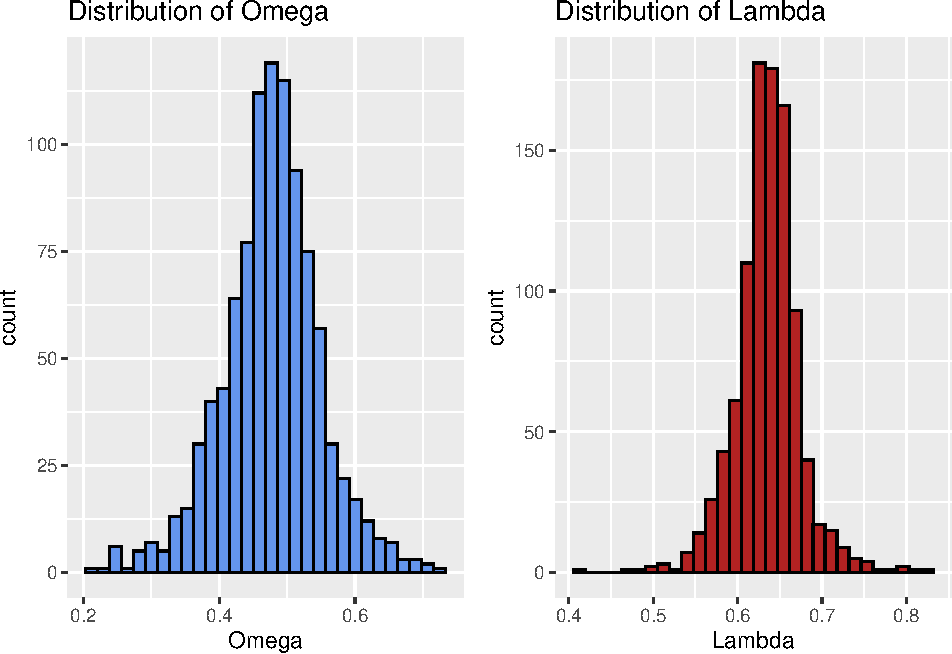
\includegraphics{Report_files/figure-latex/hists1-1.pdf}
\caption{\label{fig:hists1}Distribution of Omega and Lambda (Calculated)}
\end{figure}

Because Solomon focuses his attention on the ``Bastard Orientation,'' we'll focus mostly on \(\lambda\) here. So, let's apply this finding to the ability to predict Trump's NED vote share without specifying \(\lambda\). Our model can do this, but \emph{not} because \(\lambda\) is constant among the precincts. While the variables \(X_{bst}\) explain \emph{almost} all of the variance in the dependent variable \(\alpha_{bst}\), there are a number precincts where the OLS estimate of \(\lambda\) (hereinafter \(\hat{\lambda}\)) doesn't produce a particularly accurate prediction. We can see this by looking at the residuals of the model. The model's residuals are the difference between the actual value of \(\alpha\) from the precinct-level data and the value predicted by the OLS model (\(\hat{\alpha}_{bst}\)).

We can take a quick look at these residuals by precinct in Figure \ref{fig:residz}. Here, those precincts where the model \emph{perfectly} predicts Trump's NED vote share (\(\alpha\)) are located around the horizontal line at zero. These are in blue. As the model's estimate of a precinct's Trump NED vote share \(\hat{\alpha}_{bst}\) gets farther from the true value of that precinct's \(\alpha\), the points move farther from that line and become redder. Keep in mind, too, that the residuals are measured on the same scale as \(\alpha\), so a residual of 0.06 means that the model's estimate of Trump's NED vote share is off by 6 percentage points. Given how close the 2020 presidential race was in Nevada (Biden won with 50.06\% of the vote, with Trump earning 47.67\%), a six percentage point difference is fairly large.

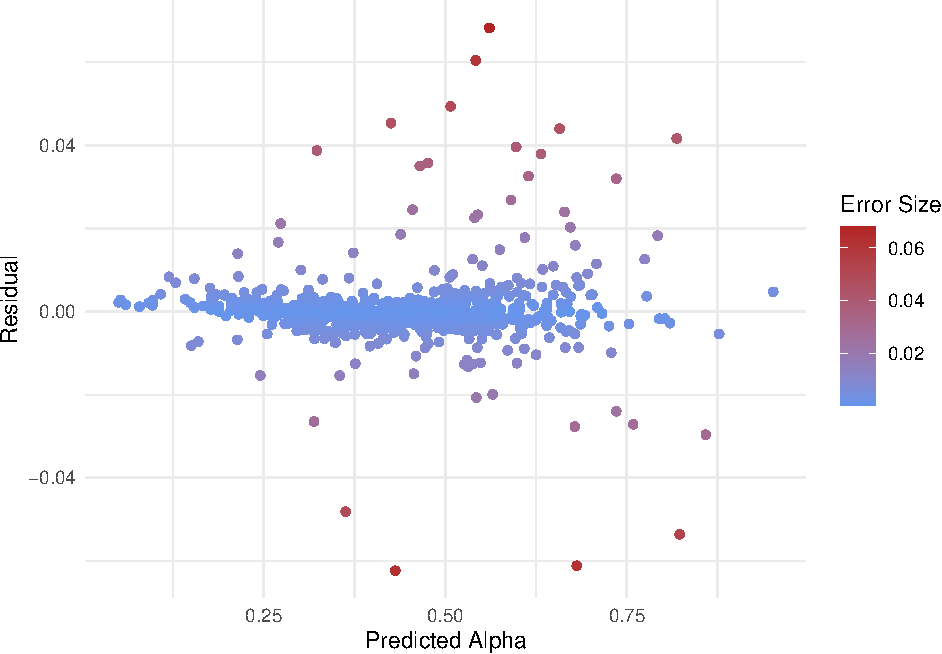
\includegraphics{Report_files/figure-latex/residz-1.pdf}

But this isn't the end of the story. Because of the way OLS regression actually works, the parameter estimates are influenced by those precincts with higher residuals. We can see this in Figure \ref{fig:infl}, which is a plot depicting the influence of each individual precinct on the estimation of the parameters \(\hat{\lambda}_{bst}\) and \(\widehat{1-\lambda}_{best}\). Here, we see a bubble chart where a monotonic transformation of the residuals is plotted against a statistic called ``leverage,'' which measures how extreme the values of \(X_{bst}\) are. The bubbles represent another statistic called ``Cook's D,'' which is the effect of each precinct's residual on the overall estimation of \(\hat{\lambda}_{bst}\) and \(\widehat{1-\lambda}_{best}\). The bigger the bubble, the more work that precinct does in pulling the parameter estimates toward its location.

\begin{figure}
\centering
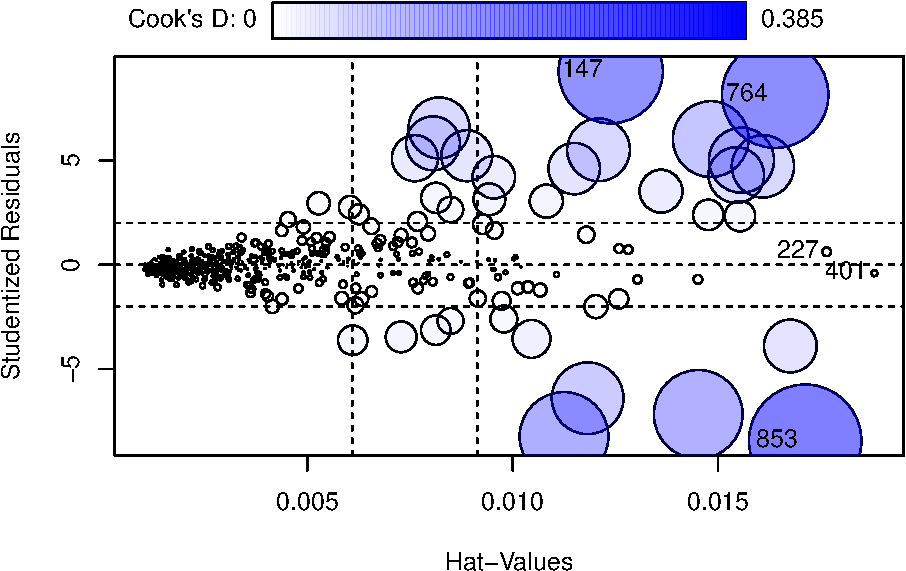
\includegraphics{Report_files/figure-latex/infl-1.pdf}
\caption{\label{fig:infl}Influence of Outliers on Lambda Estimate}
\end{figure}

This shows that, despite the fact that the parameter estimates \(\hat{\lambda}_{bst}\) and \(\widehat{1-\lambda}_{bst}\) are highly significant in the model, the model itself is definitely \emph{not} perfectly predicting Trump's share of the NED vote (\(\alpha\)) using a single value for \(\lambda\). Instead, the model is making very good (but imperfect) prediction using an estimate of \(\lambda\) that is derived from the actual patterns in the data. In short, the fact that there is a high \(R^2\) statistic for the Bastard Orientation model and the parameter estimates are statistically significant does \emph{not} mean that the relative proportion of Trump dominant votes to all dominant votes is constant across all of these precincts. As we've seen above, they aren't.

This should dispel the idea that a result like this \emph{must} mean that ballot counters have ``rigged'' the election by adding or subtracting certain votes in order to hit a certain Trump dominant to overall dominant vote ratio goal. The fact that these ratios are, in fact, different across precincts makes this argument moot. However, we do find that the values are \emph{similar} across precincts. Should that raise its own alarm bells?

\paragraph{\texorpdfstring{We Should \emph{Expect} \(\lambda\) to be Similar Across Districts.}{We Should Expect \textbackslash lambda to be Similar Across Districts.}}\label{we-should-expect-lambda-to-be-similar-across-districts.}

We've just seen that the reason we can estimate \(\alpha\) using the Standard or Bastard Orientation OLS model without including precinct-level information about the percentage of votes cast by dominant vote type is that there substantial consistency from precinct-to-precinct on this measure. This is because voters supporting a particular candidate in recent elections tend to choose similar voting methods, regardless which precinct they vote in. It's clear from the above analysis that values of \(\Omega\) and \(\lambda\) are not identical from precinct to precinct in any given election. However, should we be suspicious of similar rates of NED utilization by type and party among precincts? The research suggests that the patterns of partisan polarization we see in out data are consistent with what researchers have observed nationwide since 2020.

In essence, Solomon's argument is that the voting methods that he calls ``dominant'' for the various candidates should not be consistently dominant across precincts. Here, he's arguing that it's suspicious to find that the partisan gap in voting method would be relatively consistent across precincts in an election. A quick review of the history and the scholarly literature gives us some clarity on this issue. In short, there's no reason to expect that there should be large precinct-to-precinct variation in utilization rates for different voting methods by political party.

Nevada has a long history with NED voting methods. In fact, soldiers in the Civil War were permitted to vote on the ratification of Nevada's constitution using absentee mail ballots (Fortier and Ornstein 2003). Sick or disabled Nevadans have been allowed to vote by mail since 1921 (Ray 1924). That same law was apparently the first in the nation to allow \emph{any} ``voters who reside in precincts having less than twenty voters'' to vote by mail (or in person at the county seat on election day) (Ray 1924, 324) even if they aren't sick or disabled. Nevada also appears to be the first to allow applications for absentee ballots to ``be made by telegram'' (Ray 1924, 323). By the 1990s, Nevada joined a number of states providing the opportunity for voters to vote early in-person (Gronke, Galanes-Rosenbaum, and Miller 2007) or to request mail-in absentee ballots once identification is presented to the county election officer (Research Division 2016).

Research has been somewhat mixed on the impact of alternative voting methods on voter turnout (Gronke, Galanes-Rosenbaum, and Miller 2007). Some voters turn to alternative voting methods when they have been assigned to new precincts, although not enough to offset the abstention rate for such voters (Amos, Smith, and Ste. Claire 2017). Alternative methods do seem to be preferred when voters live far from their polling place. A study of turnout in the 2002 midterm elections in Clark County found just such an effect (Dyck and Gimpel 2005). For Nevadans who live farther from their in-person polling site, ``absentee voting through the mail increases steadily\ldots to the point where at 24 miles of distance, 30 percent of voters are mailing in their ballots'' (Dyck and Gimpel 2005, 541). This same study found that those who lived close to the early voting sites tended to use them, but ``distance from an early-voting site did not discourage voting by rather converted would-be early voters into precinct voters'' (Dyck and Gimpel 2005, 540). Overall, most of the research has showed that alternative voting methods make things easier for people who were already motivated to vote, but that they do little to increase turnout among the unengaged Karp and Banducci (2000). However, this does suggest that there may be some variations in utilization rates of mail and early voting if we are comparing precincts covering larger versus smaller geographic areas.

Before the 2020 election, there was little evidence of partisan differences in the utilization of different voting methods. An analysis of mail voting in California and Iowa found ``little or no evidence of systematic partisan skewing'' (Patterson and Caldeira 1985, 785). A study of Oregon's first all-mail election found that mail balloting did not motivate registered Republicans any differently than registered Democrats (Berinsky, Burns, and Traugott 2001). A comparison of partisanship before and after implementation of this system in Oregon showed ``the shift in balloting method was party neutral'' (Hanmer and Traugott 2004 ,394). A study of universal vote by mail elections pre-COVID in California, Utah, and Washington State similarly found no differences in party shares of turnout or vote share (Thompson et al. 2020). There is some evidence, however, suggesting that partisan mobilization efforts may impact the partisan balance of voters utilizing mail-based absentee voting (Patterson and Caldeira 1985).

The need for alternatives to election day voting became acute in the lead-up to the 2020 election, given the deadly COVID-19 pandemic. At the start of the pandemic, there was little reason to believe that alternative voting methods would become a partisan issue. In February of 2020, a team of researchers fielded a pair of surveys asking respondents which potential voting option they preferred: voting at a polling station, voting on the internet, or voting by mail (Plescia, Sevi, and Blais 2021). As the authors explain, the surveys ``took place before postal voting became a partisan issue and as such we are able to study what did people think \emph{before} the topic became controversial and highly polarized'' (Plescia, Sevi, and Blais 2021, 381). Their results found that 56\% of conservatives preferred polling stations compared to 44\% of liberals, although ``the biggest cleavage about how people should/could vote is not ideological, it is generational'' (Plescia, Sevi, and Blais 2021, 384).

Research on data predating the pandemic shows that the implementation of mail voting can cause a temporary decrease in voter confidence in the system that resolves itself after a election cycle (Clark 2021). In the early days of the pandemic, majorities of Republicans and Democrats expressed a preference for mail voting for the general election (Kousser et al. 2020). However, the months leading up to the 2020 general election provided some voters with significantly more reason for concern about health-related changes to election methods. During this time, mail voting \emph{did} become highly polarized. President Trump warned his voters about mail ballots being rife with fraud, all the while his newly-appointed Postmaster General was taking steps that appeared to be designed to ``undermine the U.S. Postal Service's\ldots capacity in an attempt to benefit President Trump's election prospects'' (Clark 2021, 382). As one study describes it,

\begin{quote}
The Center for Disease Control (CDC) encouraged voters to use, ``voting alternatives that limit the number of people you come in contact with or the amount of time you are in contact with others.'' The pandemic led Congressional Democrats to introduce legislation to expand no excuse {[}vote by mail{]} and early voting in all the states, but messages from GOP elites, especially President Trump, highlighted concerns that ballots case remotely by mail could result in lost, fraudulent, or miscounted votes\ldots.In this case, partisan-based elite messaging and polarized media content magnified the uncertainty about whether the benefits attached to voting would be realized using {[}vote by mail{]}, and this message resonated more strongly with Republicans than Democrats{]}. (Atkeson et al. 2022, 21--22)
\end{quote}

These messages appeared to hit home for Republican voters. One study found that the partisan divide in preference for voting by mail was ten points in April and had grown to twenty points just two months later (Lockhart et al. 2020). Another study found a similar trajectory in partisan polarization on the issue that continued to grow through election day (Clinton et al. 2022). A New Mexico study found ``concrete evidence of partisan polarized choices in voting behavior, even among individuals facing similar levels of risk based upon age'' (Atkeson et al. 2022, 21); registered Democrats were more likely to choose vote by mail, while Republicans were more likely to vote early in person. Evidence suggests that the partisan differences in voting method were not the ultimate driver of the outcome in the 2020 elections, as the increased utilization of mail voting among Democrats was offset by the larger share of Republicans using early or same-day voting in that election (Yoder et al. 2021).

In all, the existing research shows that there is little intrinsic partisan difference in the choice of voting methods among voters. However, it also shows the key role that elite messaging has played in adding a partisan valence to this choice. In the wake of President Trump's vocal campaign against mail voting, Republicans became far less accepting of voting by mail than did Democrats or unaffiliated voters. This pattern was replicated across a number of different studies across different legal and electoral contexts in the 2020 election. This suggests that this new partisan polarization in vote method choices is relatively consistent. Given this context, it shouldn't be surprising that the percentage of Republican voters using early in-person voting, the percentage of Democratic voters using mail voting, or any other party/method combination would be relatively constant across precincts in state-level election results.

\subsubsection{Conclusion: Vote Share Equations}\label{conclusion-vote-share-equations}

In this section, we have evaluated the claims made in the Beadles post and the work by Solomon that Beadles cites there. We have investigated the premise of the \emph{Vote Share Equations} argument and found no evidence to suggest that vote totals have been adjusted to meet a precise proportion of votes by candidate and NED vote type. Instead, we have found evidence that the OLS equations that underpin the claim that NED utilization rates by party are equal across the precincts. Instead, those models show a predictable level of consistency in utilization rates given the polarizing messages received by Republicans by their party's leader. Because Republicans were admonished against using mail ballots, it is not surprising that many of them opted for in-person early voting to avoid the risk of contracting COVID-19 at crowded election-day polling places.

\newpage

\subsection*{References}\label{references}
\addcontentsline{toc}{subsection}{References}

\hypertarget{refs}{}
\begin{CSLReferences}{1}{0}
\leavevmode\vadjust pre{\hypertarget{ref-amosReprecincting2017}{}}%
Amos, Brian, Daniel A. Smith, and Casey Ste. Claire. 2017. {``Reprecincting and Voting Behavior.''} \emph{Political Behavior} 39: 133--56.

\leavevmode\vadjust pre{\hypertarget{ref-atkesonShould2022}{}}%
Atkeson, Lonna Rae, Wendy L. Hansen, Maggie Toulouse Oliver, Cherie D. Maestas, and Eric C. Wiemer. 2022. {``Should I Vote-by-Mail or in Person? The Impact of COVID-19 Risk Factors and Partisanship on Vote Mode Decisions in the 2020 Presidential Election.''} \emph{PLOS ONE} 17 (9): e0274357. \url{https://doi.org/10.1371/journal.pone.0274357}.

\leavevmode\vadjust pre{\hypertarget{ref-berinskyPerverse2005}{}}%
Berinsky, Adam J. 2005. {``The Perverse Consequences of Electoral Reform in the United States.''} \emph{American Politics Research} 33 (4): 571--491. \url{https://journals-sagepub-com.ezproxy.library.unlv.edu/doi/10.1177/1532673X04269419}.

\leavevmode\vadjust pre{\hypertarget{ref-berinskyWho2001}{}}%
Berinsky, Adam J., Nancy Burns, and Michael W. Traugott. 2001. {``Who Votes by Mail?: A Dynamic Model of the Individual-Level Consequences of Voting-by-Mail Systems*.''} \emph{Public Opinion Quarterly} 65 (2): 178--97. \url{https://doi.org/10.1086/322196}.

\leavevmode\vadjust pre{\hypertarget{ref-clarkLost2021}{}}%
Clark, Jesse T. 2021. {``Lost in the Mail? Vote by Mail and Voter Confidence.''} \emph{Election Law Journal} 20 (4): 382--94. \url{https://heinonline.org/HOL/P?h=hein.journals/enlwjr20&i=382}.

\leavevmode\vadjust pre{\hypertarget{ref-clintonTrumped2022}{}}%
Clinton, Joshua D., John Lapinski, Sarah Lentz, and Stephen Pettigrew. 2022. {``Trumped by Trump? Public Support for Mail Voting in Response to the COVID-19 Pandemic.''} \emph{Election Law Journal: Rules, Politics, and Policy}, March. \url{https://doi.org/10.1089/elj.2020.0671}.

\leavevmode\vadjust pre{\hypertarget{ref-dyckDistance2005}{}}%
Dyck, Joshua J., and James G. Gimpel. 2005. {``Distance, Turnout, and the Convenience of Voting.''} \emph{Social Science Quarterly} 86 (3): 531--48.

\leavevmode\vadjust pre{\hypertarget{ref-Election2024}{}}%
\emph{Election Summary Report: Closed Primary, Washoe County}. 2024. Washoe County Registrar of Voters. \url{https://www.washoecounty.gov/voters/2024-election/2024-election-files/ElectionSummaryReport062024.pdf}.

\leavevmode\vadjust pre{\hypertarget{ref-fortierAbsentee2003}{}}%
Fortier, John C., and Norman J. Ornstein. 2003. {``The Absentee Ballot and the Secret Ballot: Challenges for Election Reform.''} \emph{Michigan Journal of Law Reform} 36: 483--516.

\leavevmode\vadjust pre{\hypertarget{ref-gronkeEarly2007}{}}%
Gronke, Paul, Eva Galanes-Rosenbaum, and Peter A. Miller. 2007. {``Early Voting and Turnout.''} \emph{PS: Political Science \& Politics} 40 (4): 639--45.

\leavevmode\vadjust pre{\hypertarget{ref-hanmerImpact2004}{}}%
Hanmer, Michael J., and Michael W. Traugott. 2004. {``The Impact of Voting by Mail on Voter Behavior.''} \emph{American Politics Research} 32 (4): 375--405. \url{https://doi.org/10.1177/1532673X04263412}.

\leavevmode\vadjust pre{\hypertarget{ref-karpGoing2000}{}}%
Karp, Jeffrey A., and Susan A. Banducci. 2000. {``Going Postal: How All-Mail Elections Influence Turnout.''} \emph{Political Behavior} 22 (3): 223--39. \url{https://doi.org/10.1023/A:1026662130163}.

\leavevmode\vadjust pre{\hypertarget{ref-kousserEarly2020}{}}%
Kousser, Thad, Mindy Romero, Mackenzie Lockhart, Seth Hill, and Jennifer Merolla. 2020. {``Early in the Pandemic, There Was No Partisan Divide over Preferences for Voting by Mail in the 2020 Election.''} \emph{California Journal of Politics and Policy} 12 (1): 1--8. \url{https://www.proquest.com/docview/2481239928/abstract/EB79332AD27A4A86PQ/1}.

\leavevmode\vadjust pre{\hypertarget{ref-lockhartAmerica2020}{}}%
Lockhart, Mackenzie, Seth J. Hill, Jennifer Merolla, Mindy Romero, and Thad Kousser. 2020. {``America{'}s Electorate Is Increasingly Polarized Along Partisan Lines about Voting by Mail During the COVID-19 Crisis.''} \emph{Proceedings of the National Academy of Sciences of the United States of America} 117 (40): 24640--42. \url{https://doi.org/10.1073/pnas.2008023117}.

\leavevmode\vadjust pre{\hypertarget{ref-pattersonMailing1985}{}}%
Patterson, Samuel C., and Gregory A. Caldeira. 1985. {``Mailing in the Vote: Correlates and Consequences of Absentee Voting.''} \emph{American Journal of Political Science} 29 (4): 766--88.

\leavevmode\vadjust pre{\hypertarget{ref-plesciaWho2021}{}}%
Plescia, Carolina, Semra Sevi, and André Blais. 2021. {``Who Likes to Vote by Mail?''} \emph{American Politics Research} 49 (4): 381--85. \url{https://doi.org/10.1177/1532673X211005684}.

\leavevmode\vadjust pre{\hypertarget{ref-rayAbsentVoting1924}{}}%
Ray, P. O. 1924. {``Absent-Voting Laws.''} \emph{American Political Science Review} 18 (2): 321--25.

\leavevmode\vadjust pre{\hypertarget{ref-researchdivisionPolicy2016}{}}%
Research Division. 2016. {``Policy and Program Report: Elections.''} Carson City, NV. \url{https://www.leg.state.nv.us/Division/Research/Publications/PandPReport/12-E.pdf}.

\leavevmode\vadjust pre{\hypertarget{ref-solomonFish2023}{}}%
Solomon, Edward. 2023. {``Fish Tank Paradox.''} \url{https://www.youtube.com/watch?v=BlKjF8kU7mY}.

\leavevmode\vadjust pre{\hypertarget{ref-sigmatime2024}{}}%
---------. 2024. {``Nevada 2024 Primaries: 13.4 Sigma Non-Partisan Mail-in Time Irregularity.''} Reno, NV: Operation Sunlight. \url{https://docs.google.com/document/d/1yCc91KwvNFcTlNUkfHuHTN_kdeBbeaMcxZNjkdbHFxI/edit?usp=sharing}.

\leavevmode\vadjust pre{\hypertarget{ref-thompsonUniversal2020}{}}%
Thompson, Daniel M., Jennifer A. Wu, Jesse Yoder, and Andrew B. Hall. 2020. {``Universal Vote-by-Mail Has No Impact on Partisan Turnout or Vote Share.''} \emph{Proceedings of the National Academy of Sciences of the United States of America} 117 (25): 14052--56. \url{https://doi.org/10.1073/pnas.2007249117}.

\leavevmode\vadjust pre{\hypertarget{ref-yoderHow2021}{}}%
Yoder, Jesse, Cassandra Handan-Nader, Andrew Myers, Tobias Nowacki, Daniel M. Thompson, Jennifer A. Wu, Chenoa Yorgason, and Andrew B. Hall. 2021. {``How Did Absentee Voting Affect the 2020 u.s. Election?''} \emph{Science Advances} 7 (52): eabk1755. \url{https://doi.org/10.1126/sciadv.abk1755}.

\end{CSLReferences}


\renewcommand\refname{References}
\thispagestyle{empty}
\singlespacing
\bibliographystyleapp{apsa-leeper}
\bibliographyapp{references, paperpack}

% code for the paperpack.bib file with references for 
% packages used in the paper comes from ch. 4.6 of 
% the R Markdown Cookbook by Xie, Dervieux, and Riederer
% (visited 11/6/2023) http://bookdown.org/yihui/rmarkdown-cookbook

\end{document}
